\chapter{RESULTS AND INTERPRETATIONS}
\label{chap:Results}

%%%%%%%%%%%%%%%%%%%%%%%%%%%%%%%%%%%%%%%
%%%%%%%%%%%%%%%%%%%%%%%%%%%%%%%%%%%%%%%
%%%%%%%%%%%%%%%%%%%%%%%%%%%%%%%%%%%%%%%

\section{Prediction versus observation}
\label{sec:fullCount}
After deriving estimates for all standard model backgrounds, we compare the number of 
observed events to the expected number of background events. 
The \ETmiss distributions for the full background prediction and the unblinded data are
shown in Figure~\ref{fig:FinalPlot}. Three benchmark signal models are also shown, 
corresponding to a gluino pair production simplified model 
 with gluino mass equal to 1700 GeV.

Table~\ref{tab:ExpObs} shows the expected and observed numbers of events for each bin in the signal region.
Within the uncertainties, no excess is observed with respect to the Standard Model prediction.


\begin{table}[ht]
    \caption{EXPECTED AND OBSERVED EVENTS IN THE SIGNAL REGION}
    \centering
    \begin{tabular}{ |c|c|c|c|c|c|}
        \hline
        $\ETmiss$ (GeV) & Exp. QCD & Exp. EWK &  Z$\gamma\gamma$ events  &Total exp. & Observed \\ [0.5ex]
        \hline
        $100 - 115$ & ${101.0}^{+25.8}_{-23.6}$ & 8.0 $\pm$ 2.5  & 1.3 $\pm$ 0.6 & ${ 110.3 }^{+25.9 }_{- 23.8 }$ & 65  \\
        $115 - 130$ & ${60.6}^{+ 22.7}_{-20.3}$ & 5.4 $\pm$ 1.7 & 1.1 $\pm$ 0.6 & ${ 67.1 }^{+22.7 }_{- 20.4 }$ & 26 \\
        $130 - 150$ & ${19.8}^{+ 16.0}_{-12.2}$ & 4.7 $\pm$ 1.5 & 1.1 $\pm$ 0.6 & ${ 25.7 }^{+16.1 }_{- 12.3 }$ & 17 \\
        $150 - 185$ & ${12.1}^{+ 8.2}_{-5.3}$  & 3.9 $\pm$ 1.2 & 1.3 $\pm$ 0.7 & ${ 17.3 }^{+8.3 }_{- 5.5 }$ & 13 \\
        $185 -  250$& ${2.5}^{+ 5.8}_{-2.1}$ & 3.4 $\pm$ 1.1 & 1.3 $\pm$ 0.6 & ${ 7.2 }^{+6.0 }_{- 2.5 }$ & 8  \\
        $\geq 250$  & ${13.4}^{+ 19.8}_{-12.4}$ & 2.0 $\pm$ 0.7 & 1.1 $\pm$ 0.5 & ${ 16.5 }^{+19.8 }_{- 12.4 }$ & 10 \\
        \hline
    \end{tabular}
    \label{tab:ExpObs}
\end{table}

\begin{figure*}[h]
\begin{center}
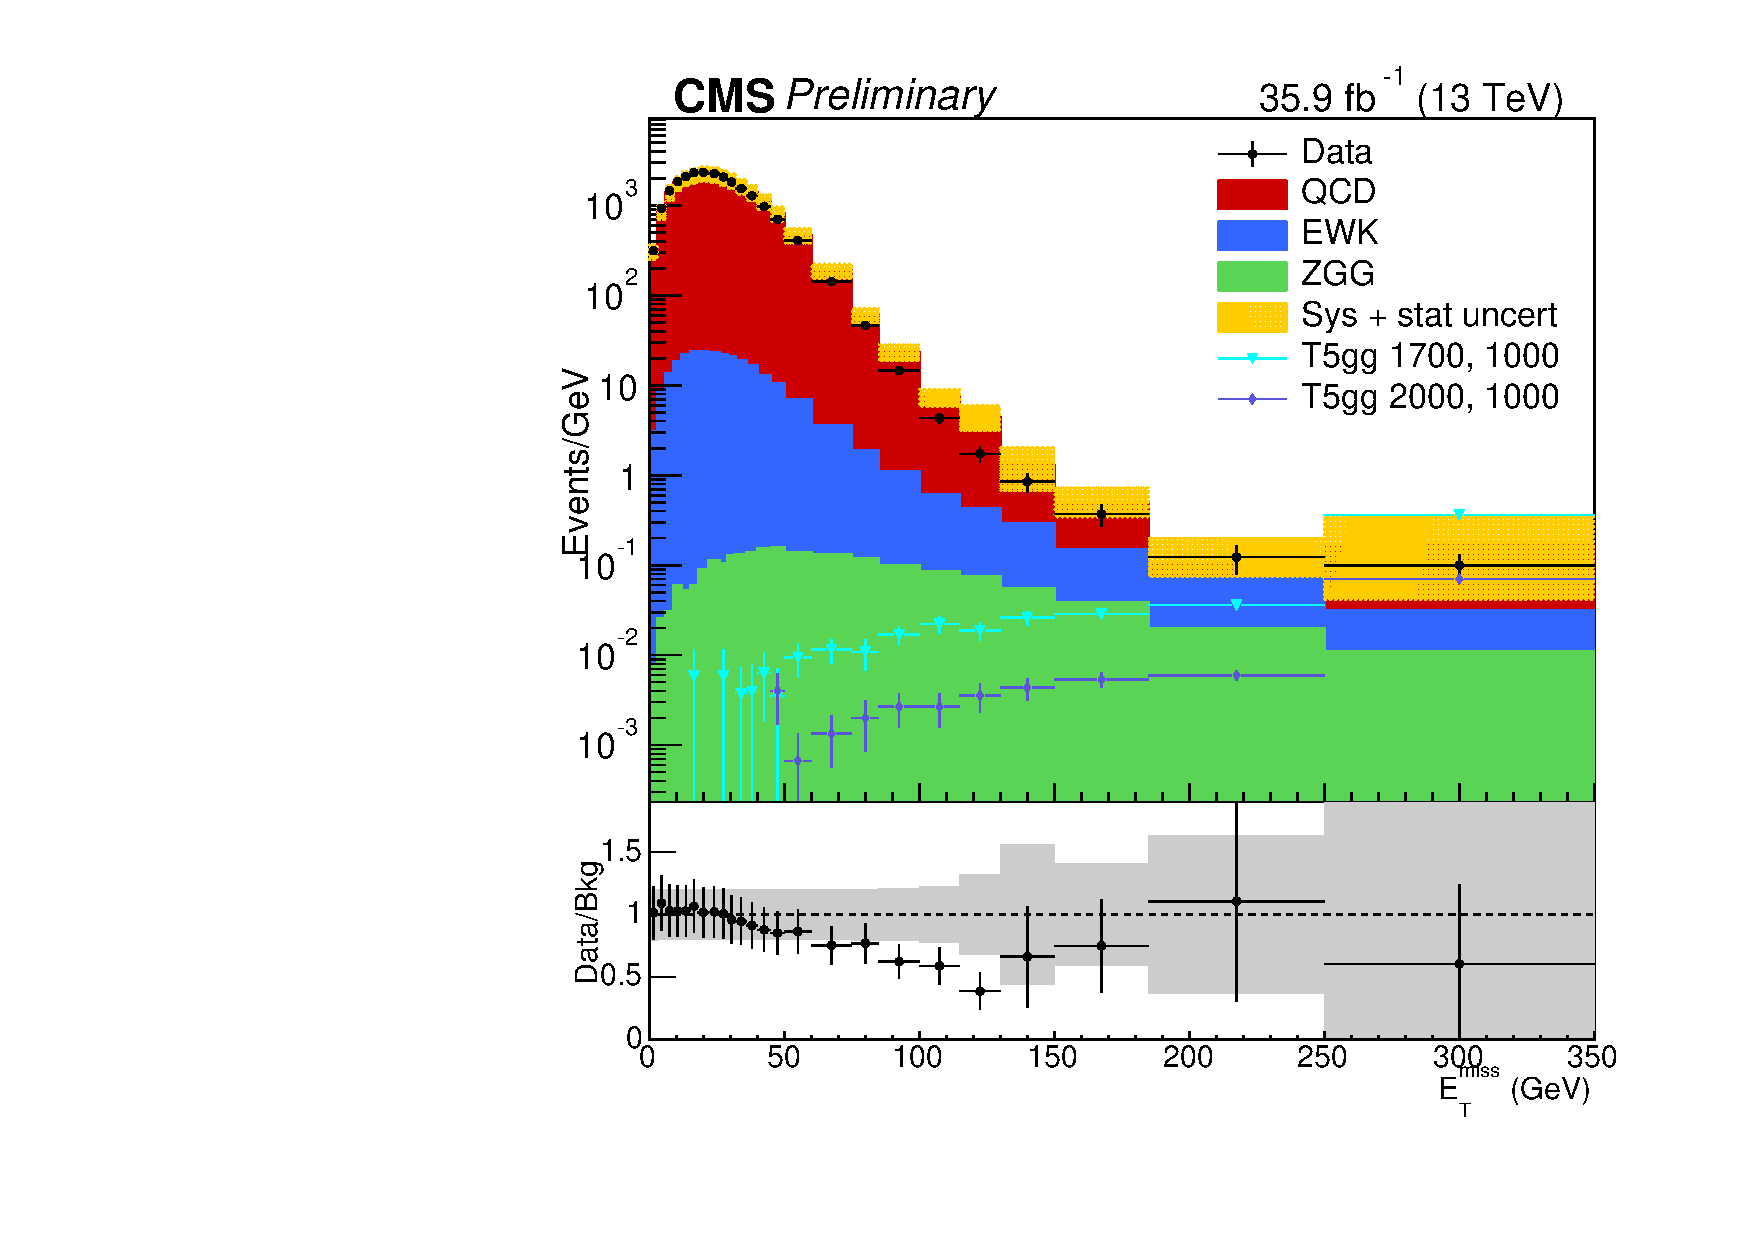
\includegraphics[width=0.9\textwidth]{Figures/Results/finalPlot.pdf}
\end{center}
\caption[\ETmiss distributions for the full background estimation and the observed data.]
{\ETmiss distributions for the full background estimation and the observed data. 
	The black points represent the observed \ETmiss distribution. 
	The QCD background (red), the EWK background
	(blue), and the $Z\gamma\gamma$ background (green) are displayed as a stacked histogram. 
	The combined uncertainty on the background estimation is shown in yellow.
	The simulated \ETmiss distributions of two benchmark T5gg mass points are displayed as well:
	the $M_{\gluino} = 1700$ GeV, $M_{\neutralino} = 1000$ GeV mass point is shown in cyan and the
	 $M_{\gluino }=$ 2000 GeV, $M_{\neutralino} = 1000$ GeV signal is shown in purple.}
\label{fig:FinalPlot}
\end{figure*}

%%%%%%%%%%%%%%%%%%%%%%%%%%%%%%%%%%%%%%%
%%%%%%%%%%%%%%%%%%%%%%%%%%%%%%%%%%%%%%%
%%%%%%%%%%%%%%%%%%%%%%%%%%%%%%%%%%%%%%%

\section{Simplified Models}
\label{sec:SimplifiedModels}

Two simplified models are used in the interpretation of the results. The T5gg simplified model assumes gluino (\gluino) pair production and the T6gg model assumes squark (\squark) pair production. Example decay chains for both models are shown in Figure~\ref{fig:gluinoSquarkDecay}.

\begin{figure*}[htbp]
    \centering
    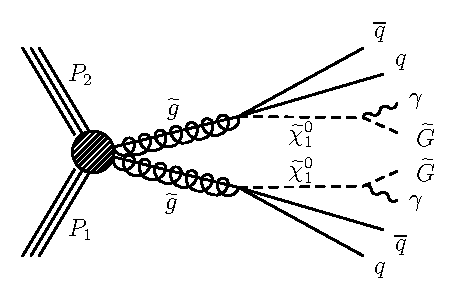
\includegraphics[width=0.45\textwidth]{Figures/Results/gluinoDecay.pdf}
    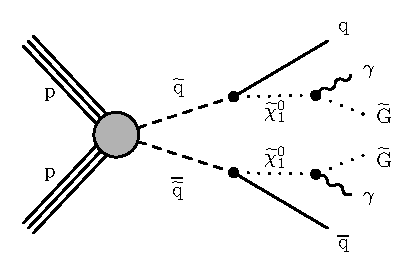
\includegraphics[width=0.45\textwidth]{Figures/Results/squarkDecay.pdf}
    \caption[Diagrams showing the production of signal events in the collision
        of two protons.]
    {Diagrams showing the production of signal events in the collision
        of two protons $p$. In gluino
        \gluino~pair production in the T5gg simplified model (left), the gluino
       decays to an antiquark \antiquark, quark q, and neutralino \neutralino. In
        squark \squark~pair production in the T6gg simplified model (right), the
        squark decays to a quark and a neutralino. In both cases, the
        neutralino subsequently decays to a photon $\gamma$~and a gravitino \gravitino.
        }
    \label{fig:gluinoSquarkDecay}
\end{figure*}

In both models, the lightest supersymmetric particle (LSP) is the gravitino, \gravitino, which is taken to be nearly massless. The next-to-lightest supersymmetric particle (NLSP) is the neutralino, \neutralino. The models assume 100\% branching fractions for 
$\neutralino\rightarrow\gravitino\gamma$ and 
$\gluino\rightarrow \mathrm{q} \antiquark \neutralino$ and 
$\squark\rightarrow \mathrm{q} \neutralino$.

In order to study the expected SUSY signal distributions, two
signal Monte Carlo scans were produced.
The T5gg scan was produced in bins of gluino mass and neutralino mass,
and the T6gg scan was produced in bins of squark mass and neutralino mass.
The leading-order event generator \textsc{MadGraph}5\_a\MCATNLO~\cite{Alwall:2014hca}
is used to simulate the signal samples, which
were generated with either two gluinos or two squarks and up to two additional
partons in the matrix element calculation. The parton showering, hadronization,
multiple-parton interactions, and the underlying event were described by the
\PYTHIA 8~\cite{Sjostrand:2007gs} program with the CUETP8M1 generator tune.
The detector response is simulated using
CMS fast simulation~\cite{Abdullin:2011zz}.

A total of 40,000 events were produced for
each bin, except for bins with gluino or squark masses above 2.0 TeV, where only
20,000 events were produced per bin.
For gluino masses from 1,400 to 2,500 GeV, events were generated
in bins of 50 GeV.  In the T6gg scan, the squark masses ranged from
1,400 GeV to 2,050 GeV in bins of 50 GeV.
The neutralino masses ranged from 10 GeV up to the mass
of the gluino or squark and were binned in
100 GeV segments. Finer binning was used in the compressed region where
$M_{\neutralino}$ is within 300 GeV of $M_{\gluino}$ or $M_{\squark}$,
and in the region with low $M_{\neutralino}$.
These mass ranges were selected to overlap and
expand upon the mass ranges excluded by previous
searches~\cite{ATLAS:2016aa,CMS:2015_anal}.

The parton distribution
functions are obtained from NNPDF3.0~\cite{Ball:2014uwa}.
Figure~\ref{fig:xSec} shows the cross sections as a function
of squark and gluino mass.
The cross sections are calculated at next-to-leading order 
(NLO) accuracy including the resummation of soft gluon emission
at next-to-leading-logarithmic (NLL) accuracy~\cite{Kulesza:2009kq, Beenakker:2009ha},
with all the unconsidered sparticles assumed to be heavy and decoupled.
The uncertainties on the cross sections are calculated as
described in Reference~\cite{Borschensky:2014cia}.


\begin{figure*}[htbp]
    \centering
    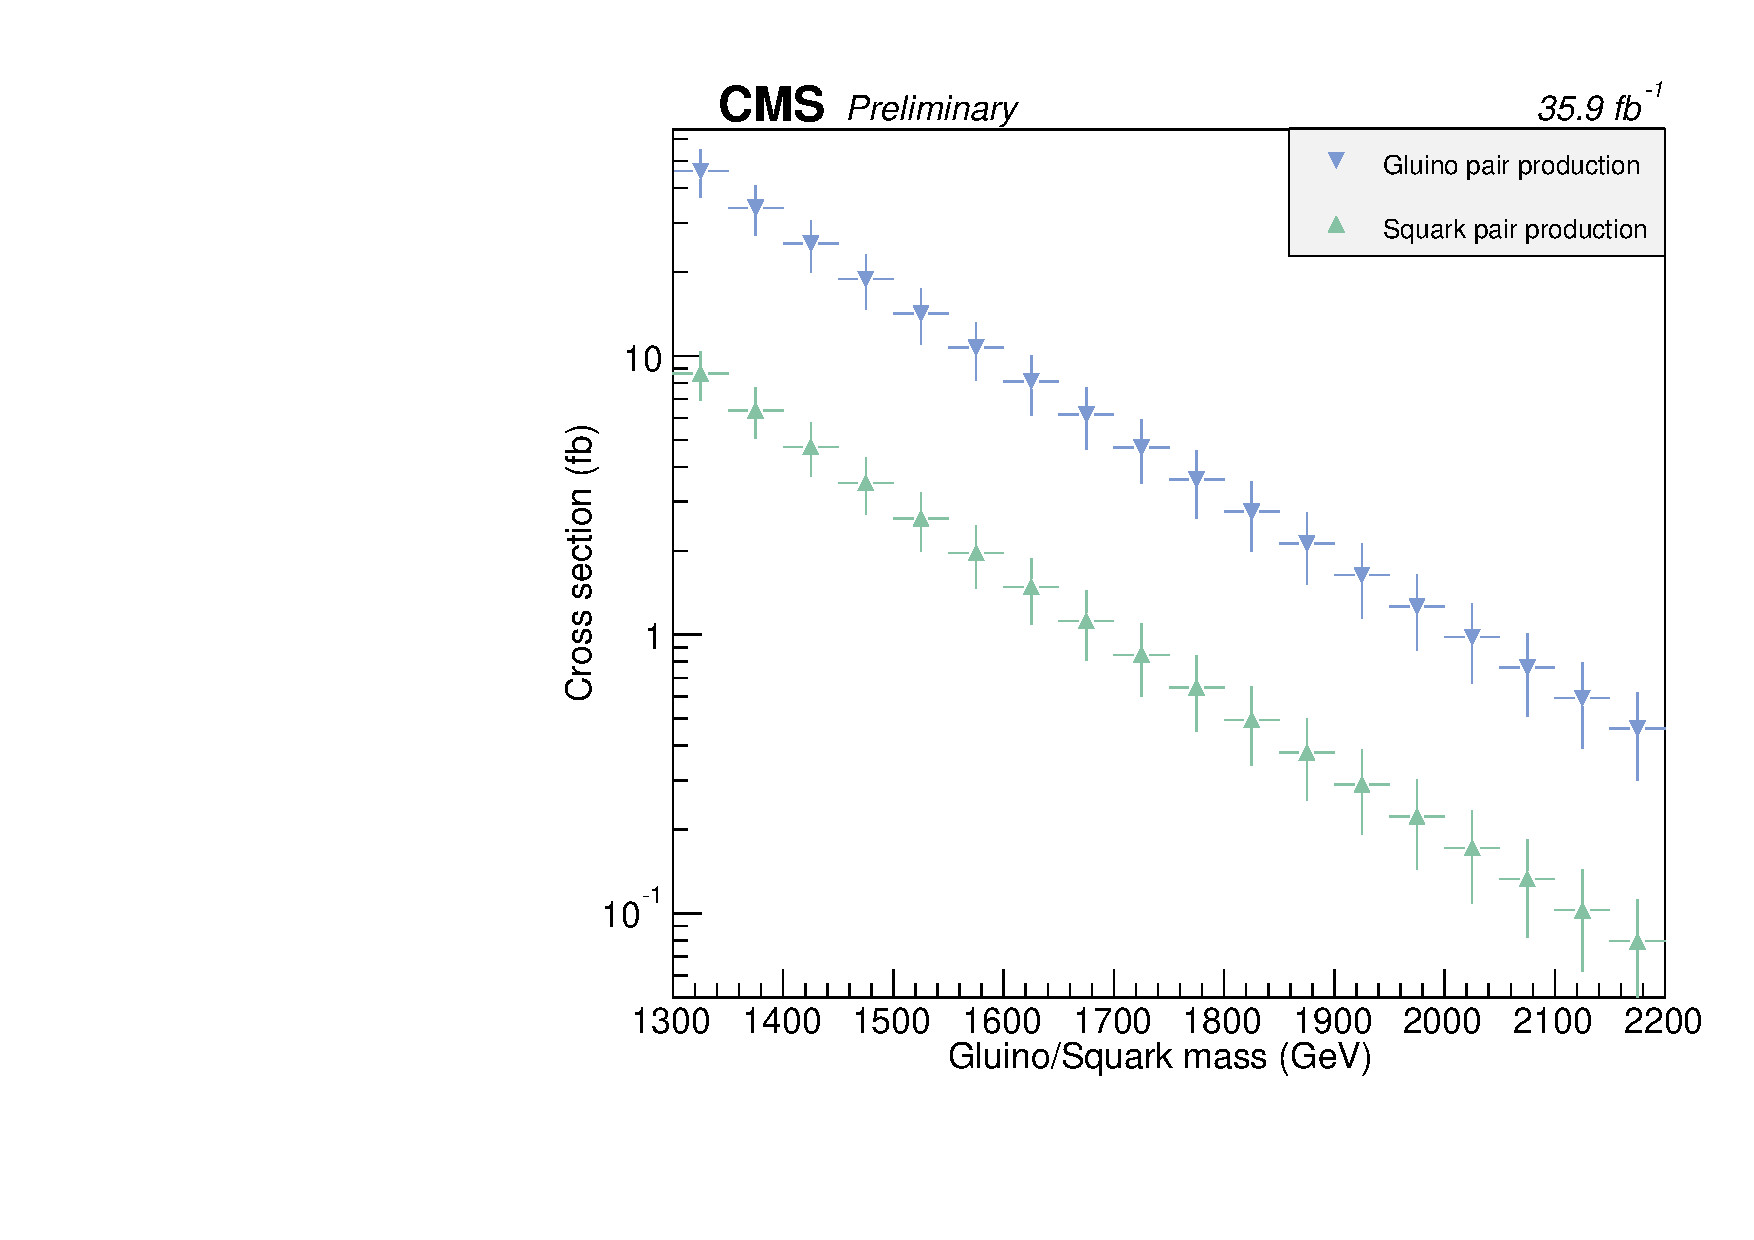
\includegraphics[width=0.8\textwidth]{Figures/Results/xSecPlot.pdf}
    \caption[NLO+NLL cross sections for the simplified gluino pair production
    and squark pair production models used in this analysis.]
    {NLO+NLL cross sections for the simplified gluino pair production (blue)
    and squark pair production (green) models used in this analysis.}
    \label{fig:xSec}
\end{figure*}

%%%%%%%%%%%%%%%%%%%%%%%%%%%%%%%%%%%%%%%

\section{Signal acceptance and efficiency}
The generated SUSY signal events undergo the same event selection described in Chapter~\ref{chap:EventSelect}. 
For every mass point, the number of events expected in each of the six signal region bins is calculated. 
In addition, the overall acceptance $\times$ efficiency ($A \times \epsilon$), defined as the number of events
passing the full $\gamma\gamma$ selection divided by the total number of generated events, is calculated across the 
full 2D mass plane. Figures~\ref{fig:accXeff_T5gg} and~\ref{fig:accXeff_T6gg} show the $A \times \epsilon$ distributions for the T5gg and T6gg simplified model 
frameworks.

\begin{figure*}[h]
\begin{center}
\includegraphics[width=0.8\textwidth]{Figures/Results/accXeff_T5gg.pdf}
\end{center}
    \caption{Acceptance $\times$ efficiency for the T5gg simplified model.}
    \label{fig:accXeff_T5gg}
\end{figure*}

\begin{figure*}[h]
\begin{center}
\includegraphics[width=0.8\textwidth]{Figures/Results/accXeff_T6gg.pdf}
\end{center}
    \caption{Acceptance $\times$ efficiency for the T6gg simplified model.}
    \label{fig:accXeff_T6gg}
\end{figure*}

%% XX Note when making this plot: numerator should technically only include the number of gg events with MET > 100 GeV XX %%
%% XX Also label palette/z-axis XX %% 

At low neutralino mass, the $A \times \epsilon$ decreases because the photons are softer and more likely to fail the \pT $> 40$ GeV cut or the 
$m_{\gamma\gamma} > 105$ GeV cut.
There is also more jet energy at low neutralino masses, which increases the chance that photons will overlap with a jet and fail the 
isolation requirements.

%%%%%%%%%%%%%%%%%%%%%%%%%%%%%%%%%%%%%%%
%%%%%%%%%%%%%%%%%%%%%%%%%%%%%%%%%%%%%%%
%%%%%%%%%%%%%%%%%%%%%%%%%%%%%%%%%%%%%%%


\section{Limits and interpretations}
\label{sec:limits}

As shown in Table~\ref{tab:ExpObs}, the observed number of events is consistent with (or less than) the total number of 
expected background events in each bin in the signal region. In the absence of a signal, these results can 
be used to set limits on the allowed squark, gluino, and neutralino masses in the T5gg and T6gg simplified models.

\subsection{Statistical analysis}
\label{sec:stats}

The probability $P$ of observing $n$ events if we expect $s$ signal events and $b$ background events
in a given bin or channel
can be expressed using a Poisson distribution:
\begin{equation}
P(n|\mu, \bm{\theta}) = \frac{(\mu s(\bm{\theta})+b(\bm{\theta}))^ne^{-\mu s(\bm{\theta})-b(\bm{\theta})}}{n!}
\end{equation}
The expected number of signal events is parameterized with a \textit{signal strength modifier} $\mu$, where $\mu = 1$ 
corresponds to the  nominal cross section. The systematic and statistical uncertainties described in 
Chapter~\ref{chap:DataAnalysis} are treated as nuisance parameters,
and their effects on $s$ and $b$ are encoded in the parameter set $\bm{\theta}$.
%probabilities of nuisances

Each nuisance parameter $\theta_i$ must have an associated probability distribution $p_i(\theta)$.
The statistical uncertainties are modeled with gamma distributions, where $x$ is the expected event yield, 
$\alpha$ is the original number of events in the control sample, 
and $\beta$ is the transfer factor, $\beta$ = $x$/$\alpha$: 
\begin{equation}
p(\theta) =	\dfrac{\beta^\alpha}{\Gamma(\alpha)} x^{\alpha-1}e^{-\beta x}
\end{equation}
The statistical uncertainties include those on the 
observed number of events in the signal region in data, uncertainties from the limited number of events
in the control regions used for the data-driven background estimation methods, and the MC statistical uncertainties 
in the SUSY signal MC and the MC used to model the $Z\gamma\gamma\rightarrow\nu\nu\gamma\gamma$ 
background.

All of the systematic uncertainties described in Chapter~\ref{chap:DataAnalysis} are constrained
with log-normal probability distributions. The peak of the probability distribution 
is set to the nominal background estimate for that bin, and the size of the systematic uncertainty 
sets the width of the distribution. 

To combine several channels or bins---in our case, the six signal bins for \ETmiss $> 100$ GeV---the 
probabilities are combined into a \textit{likelihood function} $\mathcal{L}$. The likelihood is
the probability of having a signal strength $\mu$ and nuisance parameters $\bm{\theta}$ given the observed
number of events in each bin, $\bm{n} = \{n_1,n_2,...n_i\}$:
 \begin{equation}
 \mathcal{L}(\mu, \bm{\theta}|\bm{n}) = \prod_i P(n_i|\mu,\bm{\theta})  \prod_jp_j(\bm{\theta})
 \label{equ:likelihood}
 \end{equation}
Maximizing $\mathcal{L}$ gives us the best fit values for the signal strength and nuisance parameters, referred to
as $\hat{\mu}$ and $\bm{\hat{\theta}}$, respectively.

To describe how compatible a given value of $\mu$ is with the observed data, we use the following test statistic:
\begin{equation}
t_\mu = -2 \ln{ \frac{\mathcal{L}(\mu,\bm{\tilde{\theta}})}{\mathcal{L}(\hat{\mu},\bm{\hat{\theta}})} }
\end{equation}
where $\bm{\tilde{\theta}}$ is the value of the nuisance parameters that maximizes $\mathcal{L}(\mu)$. Larger 
values of $t_\mu$ represent increased tension between $\mu$ and the observed data. 

The probability of getting a value for $t_\mu$ larger than what was actually observed is known as the $p$-value, 
$p_\mu$. If $p_{\mu=1}$ is less than 0.05, then we say that we have excluded the signal hypothesis at a 95\% 
\textit{confidence level}. In order to claim a discovery, the convention in high energy physics is to require
$p_{\mu =0} < 2.87 \times 10^{-7}$, which corresponds to 5$\sigma$ in a Gaussian distribution. 

In this analysis, we use the standard \cls method \cite{Junk:1999kv, Read:2002hq} to 
determine 95\% confidence level intervals for the cross section times branching fraction in each mass bin.
The \cls method avoids over-estimating the limits in the case of downward fluctuations in data by
normalizing the $p$-value for the signal plus background hypothesis ($CL_{s+b} = p_{\mu=1}$) to the
probability of the background-only hypothesis ($CL_{b} = p_{\mu=0}$):
\begin{equation}
CL_s = \frac{CL_{s+b}}{CL_{b}}.
\end{equation}
If $1 - \cls \leq 0.95$, then we have excluded the signal hypothesis at a 95\% confidence level.

\subsection{T5gg and T6gg limits}
\label{sec:limitResults}

The final cross section limits and exclusion contours are shown in Figure~\ref{fig:limit_T5gg} for the T5gg simplified model
and Figure~\ref{fig:limit_T6gg} for the T6gg simplified model.
In both models, the cross section is independent of the mass of the neutralino and 
depends only on the mass of the gluino or squark. Therefore, it is not surprising that the exclusion contours
do not depend sensitively on the mass of the neutralino. 

\begin{figure*}[h]
\begin{center}
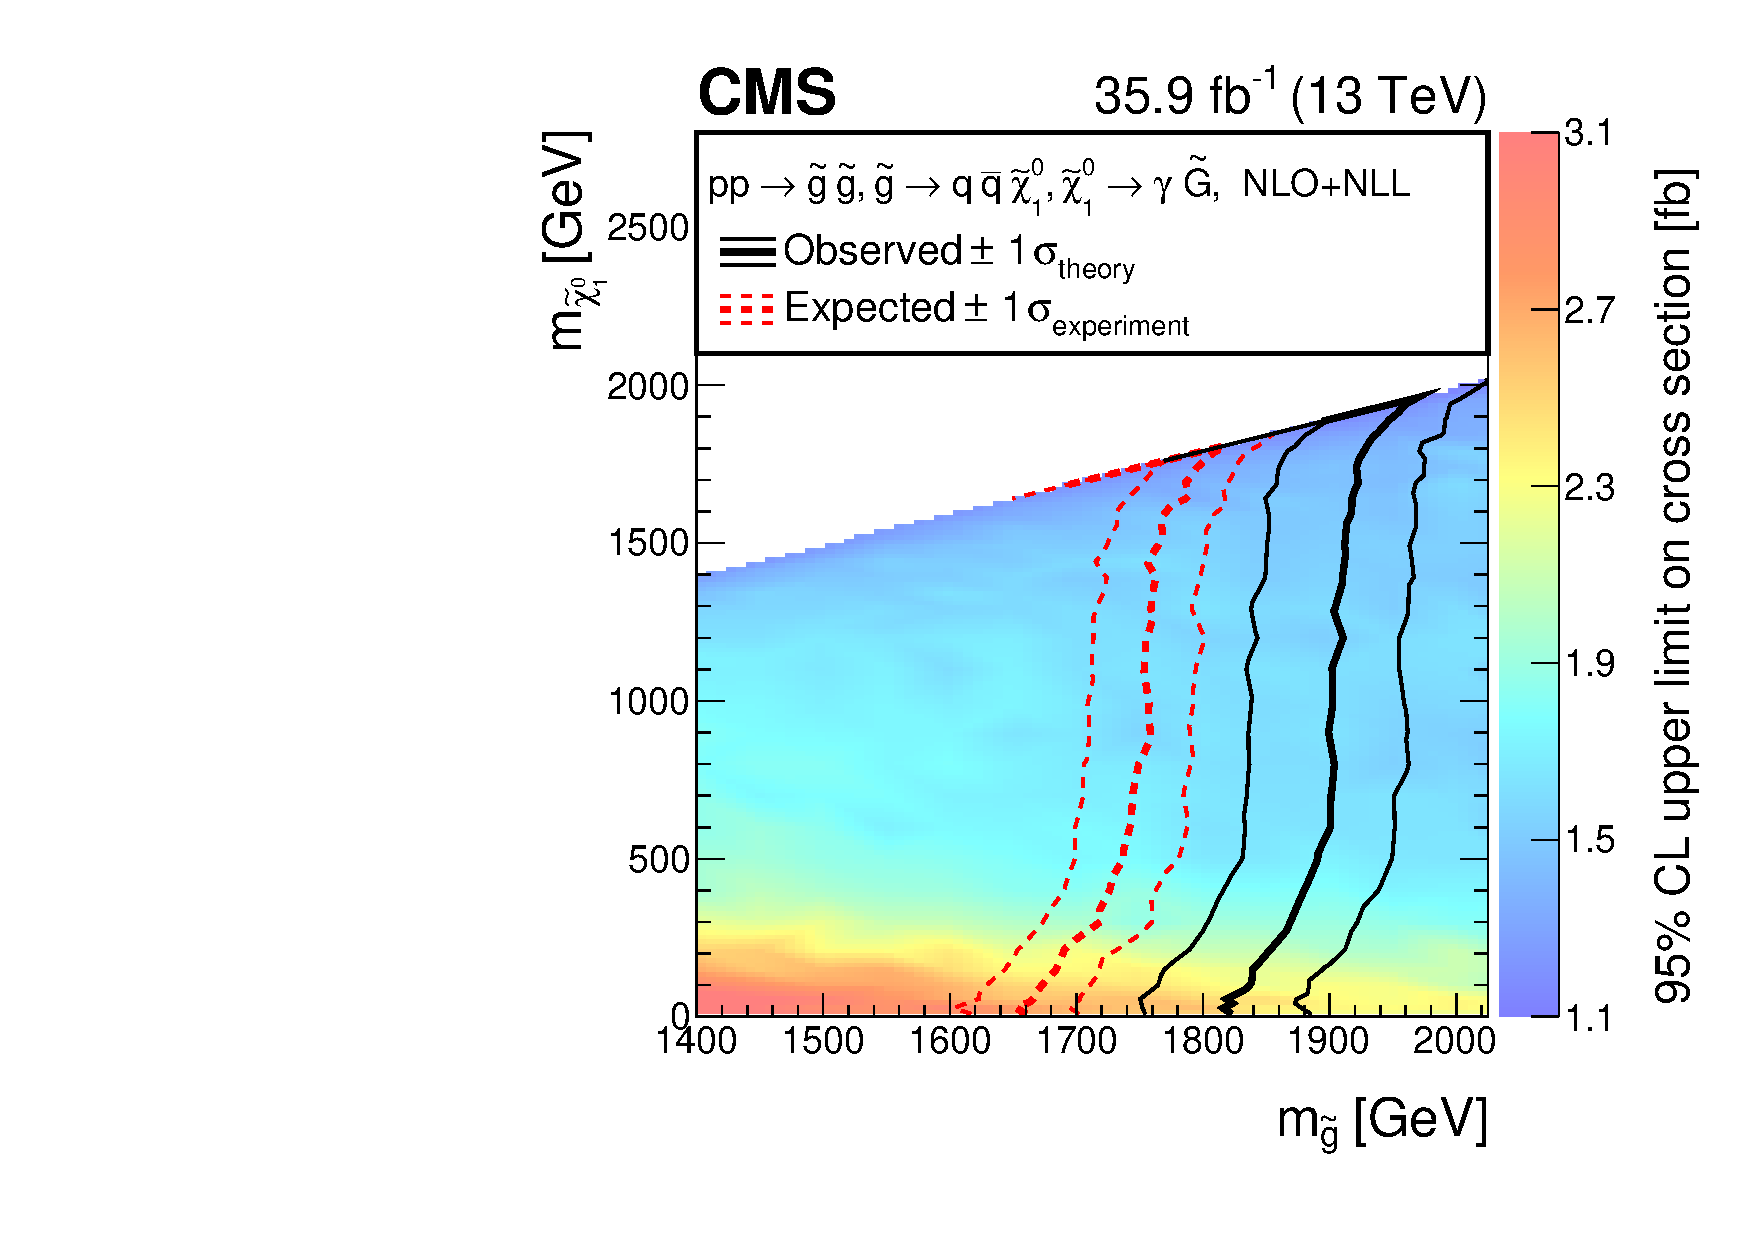
\includegraphics[width=0.7\textwidth]{Figures/Results/T5ggXSEC.pdf}
\end{center}
    \caption[The 95\% confidence level upper limits on the gluino pair
        production cross sections as a function of gluino and neutralino masses.]
    {The 95\% confidence level upper limits on the gluino pair
        production cross sections as a function of gluino and neutralino masses.
        The contours show the observed and median expected exclusions assuming
        the NLO + NLL cross sections, with their one standard deviation
	uncertainties.}
    \label{fig:limit_T5gg}
\end{figure*}

\begin{figure*}[h]
\begin{center}
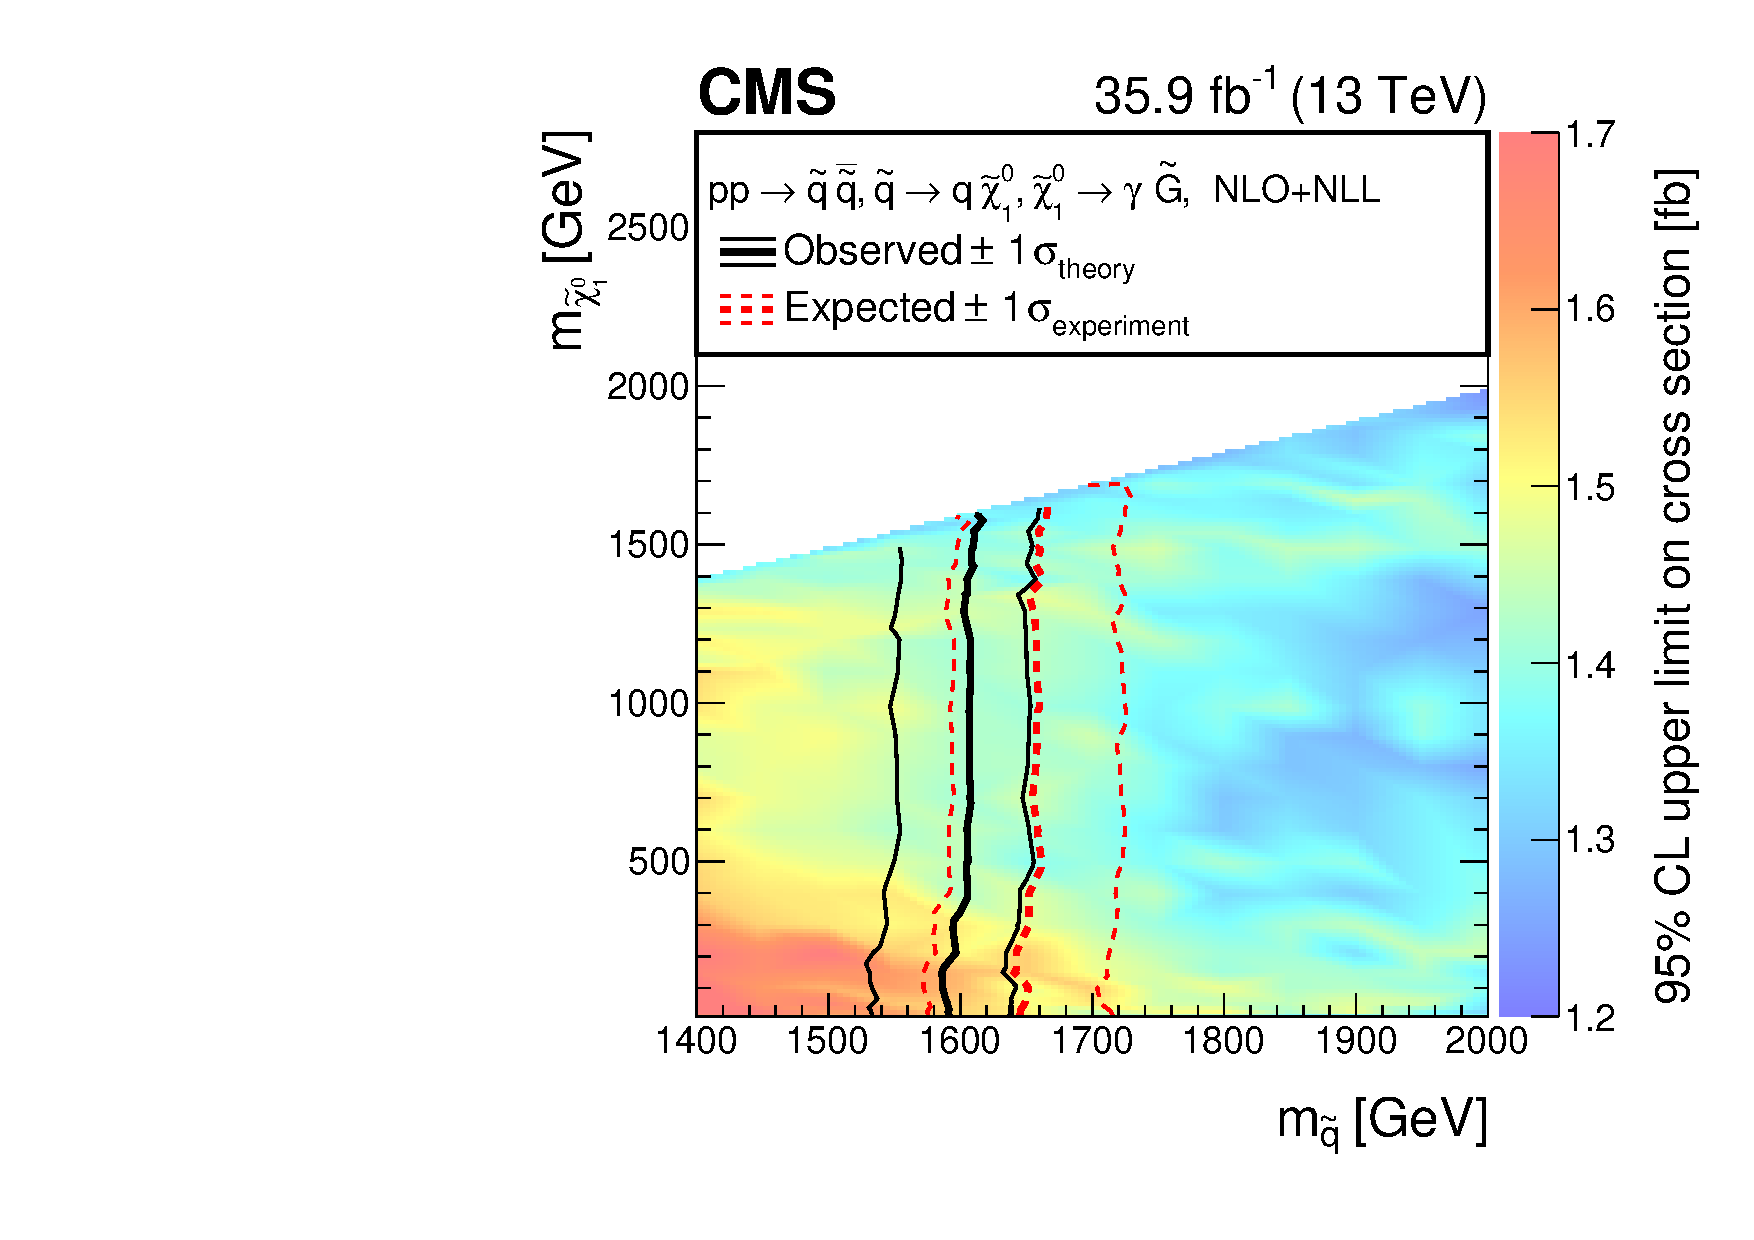
\includegraphics[width=0.7\textwidth]{Figures/Results/T6ggXSEC.pdf}
\end{center}
    \caption[The 95\% confidence level upper limits on the squark pair
        production cross sections as a function of squark and neutralino masses.]
    {The 95\% confidence level upper limits on the squark pair
        production cross sections as a function of squark and neutralino masses.
        The contours show the observed and median expected exclusions assuming
        the NLO + NLL cross sections, with their one standard deviation
	uncertainties.}
    \label{fig:limit_T6gg}
\end{figure*}

In both the T5gg and T6gg simplified models, the cross section is independent of the mass of the neutralino and 
depends only on the mass of the gluino or squark, respectively. Therefore, it is not surprising that the exclusion contours
shown in Figures~\ref{fig:limit_T5gg} and~\ref{fig:limit_T6gg}
do not depend sensitively on the mass of the neutralino. 

In the bulk of the distribution, gluino masses below 1.90 TeV and squark masses below 
1.62 TeV are excluded at a 95\% confidence level. The expected exclusions were
1.75 TeV for gluino pair production and 1.58 TeV for squark pair production. 
This is a large jump in sensitivity compared to the 2015 ATLAS and CMS results, which excluded 
masses less than 1.65 TeV and 1.37 TeV for gluinos and squarks, respectively. 

%%%%%%%%%%%%%%%%%%%%%%%%%%%%%%%%%%%%%%%
%%%%%%%%%%%%%%%%%%%%%%%%%%%%%%%%%%%%%%%
%%%%%%%%%%%%%%%%%%%%%%%%%%%%%%%%%%%%%%%

